\begin{figure}[t]
\centering

\includegraphics[width=0.8\linewidth]{sidekick/figures/cwnd_legend.pdf}\\
\begin{subfigure}{0.32\linewidth}
  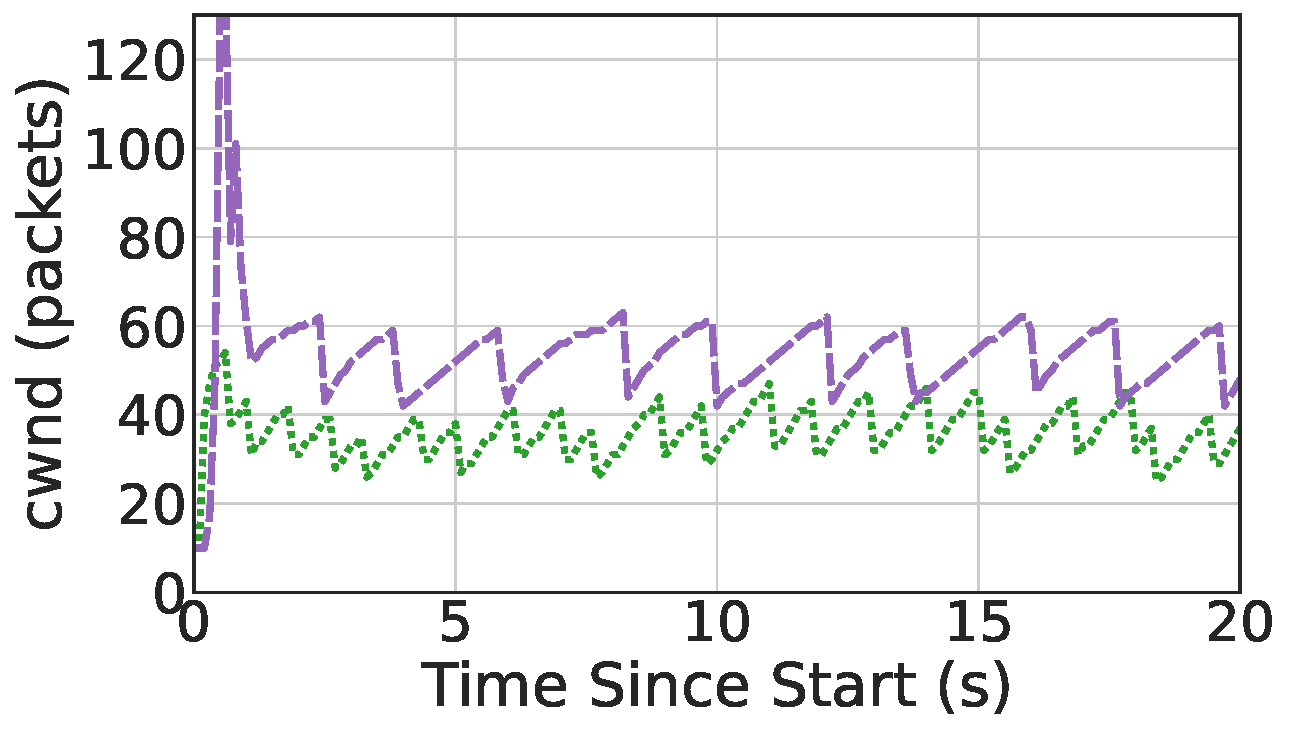
\includegraphics[width=\linewidth]{sidekick/figures/cwnd_split_loss0p.pdf}
  \caption{Split CUBIC, 0\% loss.}
  \label{fig:sidekick:pacubic:split-loss0p}
\end{subfigure}
\begin{subfigure}{0.32\linewidth}
  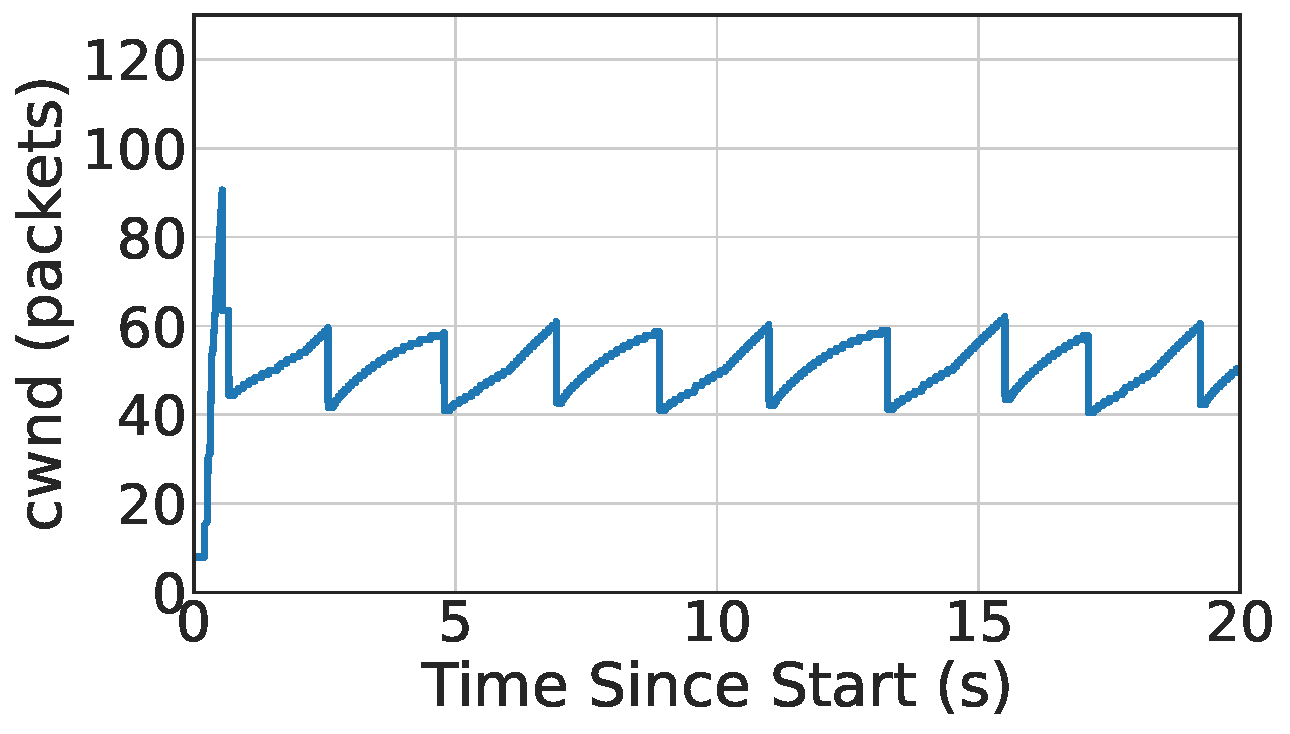
\includegraphics[width=\linewidth]{sidekick/figures/cwnd_pacubic_loss0p.pdf}
  \caption{PACUBIC, 0\% loss.}
  \label{fig:sidekick:pacubic:pacubic-loss0p}
\end{subfigure}
\begin{subfigure}{0.32\linewidth}
  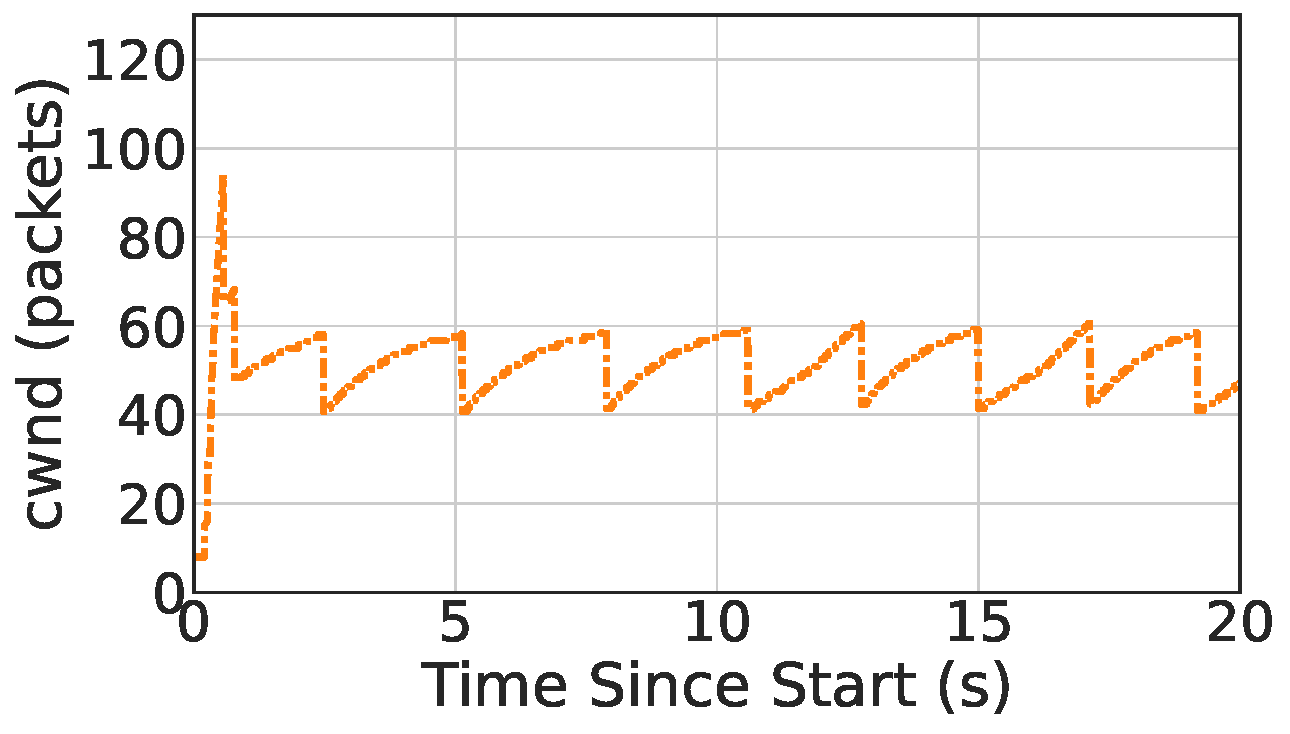
\includegraphics[width=\linewidth]{sidekick/figures/cwnd_cubic_loss0p.pdf}
  \caption{CUBIC, 0\% loss.}
  \label{fig:sidekick:pacubic:cubic-loss0p}
\end{subfigure}
\begin{subfigure}{0.32\linewidth}
  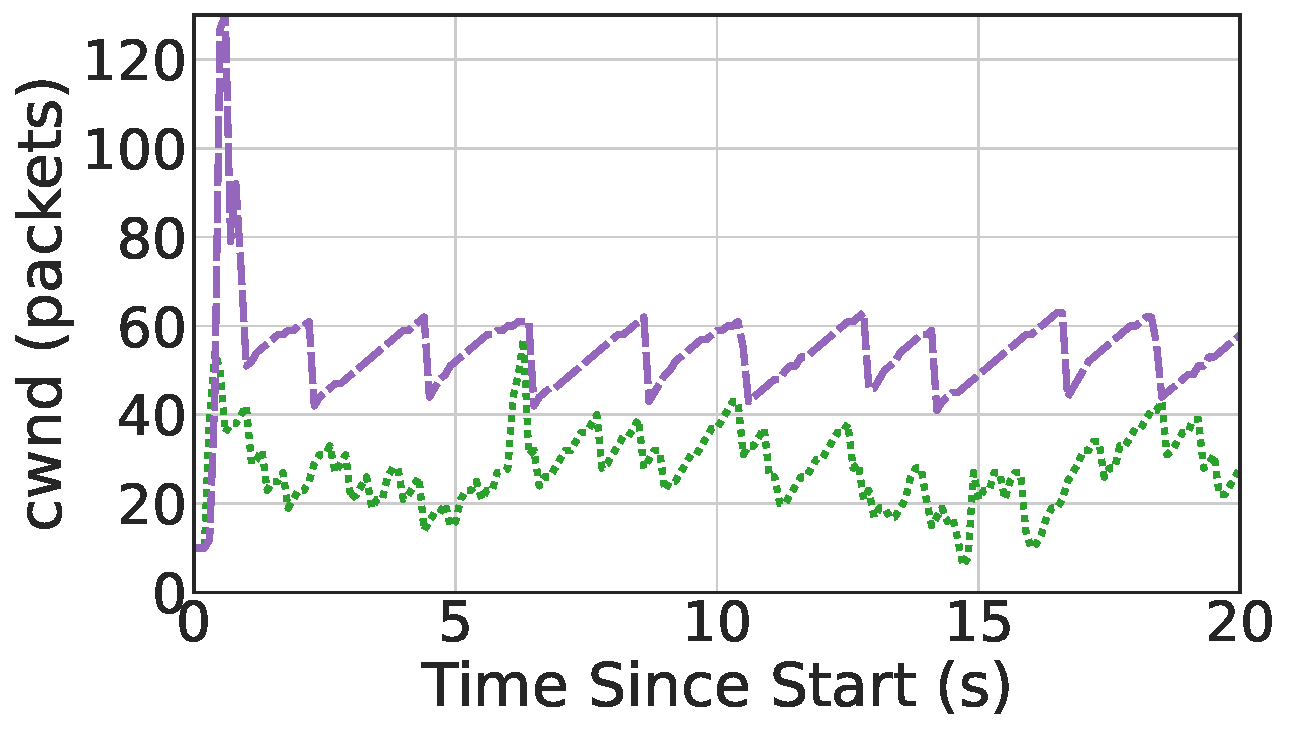
\includegraphics[width=\linewidth]{sidekick/figures/cwnd_split_loss1p.pdf}
  \caption{Split CUBIC, 1\% loss.}
  \label{fig:sidekick:pacubic:split-loss1p}
\end{subfigure}
\begin{subfigure}{0.32\linewidth}
  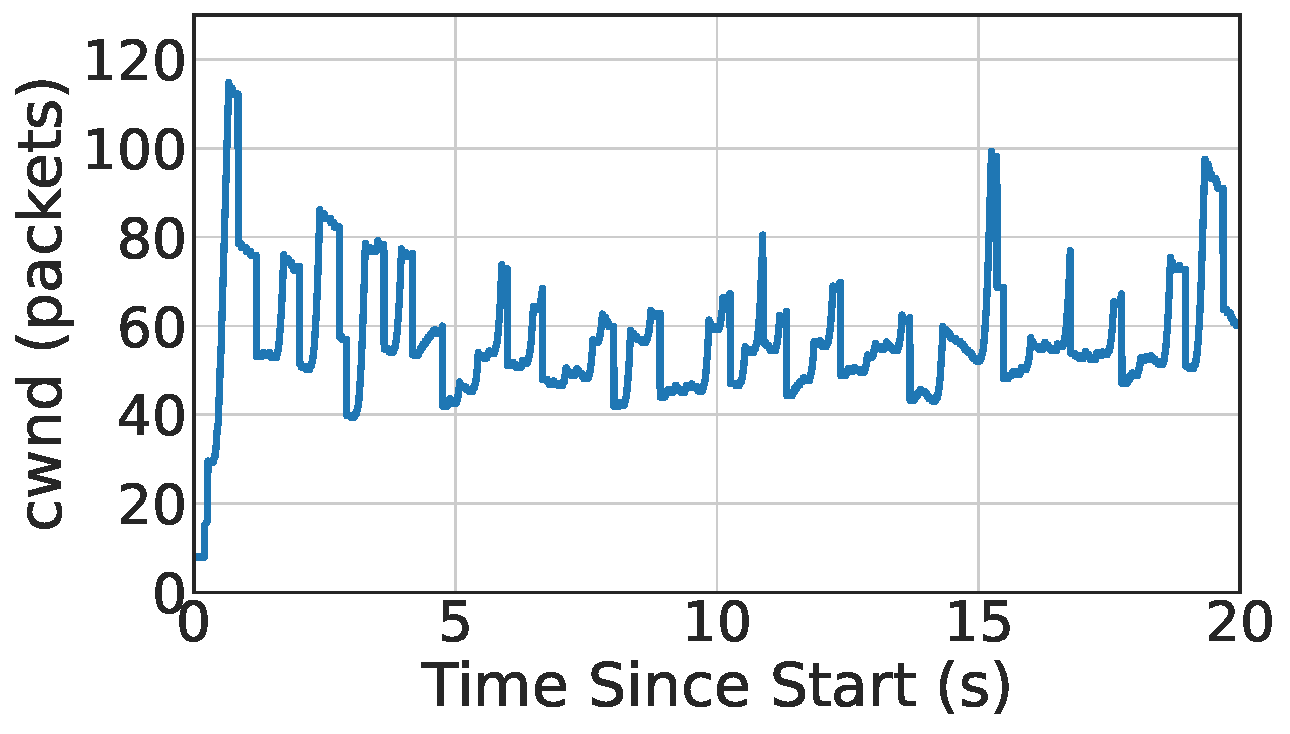
\includegraphics[width=\linewidth]{sidekick/figures/cwnd_pacubic_loss1p.pdf}
  \caption{PACUBIC, 1\% loss.}
  \label{fig:sidekick:pacubic:pacubic-loss1p}
\end{subfigure}
\begin{subfigure}{0.32\linewidth}
  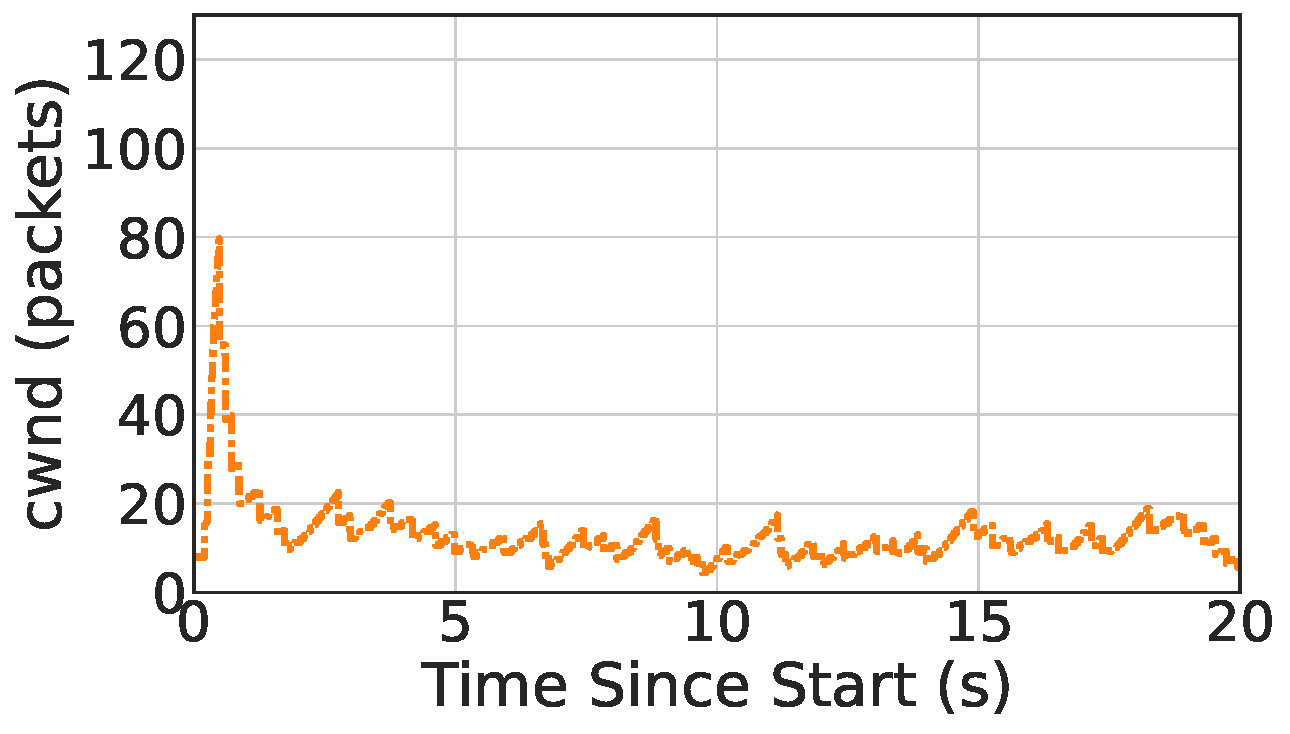
\includegraphics[width=\linewidth]{sidekick/figures/cwnd_cubic_loss1p.pdf}
  \caption{CUBIC, 1\% loss.}
  \label{fig:sidekick:pacubic:cubic-loss1p}
\end{subfigure}
\caption{Congestion window of a long-running upload in Scenario \#2
(\Cref{tab:sidekick:experimental-scenarios}) with $0\%$ and $1\%$ loss on the
near path segment. The cwnd is measured at the data sender,
except for split CUBIC whose split connection also has a cwnd at the proxy.
PACUBIC reacts to every congestion event while keeping the cwnd high.
CUBIC performs poorly when there is loss on the near path segment.
CUBIC and PACUBIC are implemented in QUIC, while split CUBIC is implemented
in TCP using a PEP.
}
\label{fig:sidekick:pacubic}
\end{figure}
